\part{Graph and Network Theory}
	\chapter{Graph Theory}
		\section{Basic concepts}
		A \textbf{Graph} G consists of a finite set $V(G)$ on vertices, a finite set $E(G)$ on edgesand an \textbf{incident relation} than associates with any edge $e\in E(G)$ an unordered pair of vertices not necessarily distinct called \textbf{ends}.

		\begin{figure}[h!]
			\centering
			\begin{tikzpicture}[node distance = 2cm]
				\node (v_2) [circleNode] {$v_2$};
				\node (v_3) [circleNode, right of = v_2] {$v_3$};
				\node (v_1) [circleNode, below of = v_2] {$v_1$};
				\node (v_4) [circleNode, below of = v_3] {$v_4$};
				\node (v_5) [circleNode, right of = v_3] {$v_5$};
				\node (v_6) [circleNode, below of = v_5] {$v_6$};
				\draw [link] (v_2) -- node [left] {$e_1$} (v_1);
				\draw [link] (v_2) -- node [below] {$e_2$} (v_4);
				\draw [link] (v_1) to [out = 180, in = 270, looseness = 5] node [right] {$e_3$} (v_1);
				\draw [link] (v_2) to [out = 45, in = 135] node [above] {$e_4$} (v_3);
				\draw [link] (v_2) to [out = 315, in = 225] node [above] {$e_5$} (v_3);
				\draw [link] (v_3) -- node [right] {$e_6$} (v_4);
				\draw [link] (v_5) -- node [right] {$e_7$} (v_6);
			\end{tikzpicture}			
		\end{figure}

		It can be represented as
		\begin{align}
			V = V(G) = \{v_1, v_2, v_3, v_4, v_5, v_6\} \\
			E = E(G) = \{e_1, e_2, e_3, e_4, e_5, e_6, e_7\}\\
			e_1 = v_1v_2, e_2 = v_2v_4, ...
		\end{align}

		Serveral concepts: \\
		\indent - An edge with identical ends is called a \textbf{loop}\\
		\indent - Two edges having the same ends are said to be \textbf{parallel}\\
		\indent - A graph without loops or parallel edges is called \textbf{simple graph}\\
		\indent - two edges of a graph are \textbf{adjancent} if they have a common end\\
		\indent - two vertices are \textbf{adjancent} if they are jointed by an edge\\
		

	\section{Subgraph}
		Given two graphs \textbf{G} and \textbf{H}, \textbf{H} is a \textbf{subgraph} of \textbf{G} if $V(H)\subseteq V(G)$, $E(H)\subseteqe E(G)$ and an edge has the smae ends in \textbf{H} as it does in \textbf{G}, if $E(H)\neq E(G)$ then \textbf{H} is a proper subgraph.

		A subgraph \textbf{H} on \textbf{G} is \textbf{spanning} if $V(H) = V(G)$

		For a subset $V^{'}\subseteq V(G)$ we define an \textbf{vertex-induced} subgraph $G[V^{'}]$ to be the subgraph with vertices $V^{'}$ and those edges of \textbf{G} having both ends in $V^{'}$

		The \textbf{edge-induced} subgraph $G[E^{'}]$ has edges $E^{'}$ and those vertices of \textbf{G} that are ends to edges in \textbf{$E^{'}$}

		If we combine node-indeced or edge-induced subgraphs $G(V^{'})$ and $G(V - V^{'})$, we cannot get the entire graph.

		Let $v\in V(G)$, then the \textbf{degree} of $v\in V(G)$ denote by $d_G(v)$ is defines to be the number of edges incident of $v$. Loops counted twice.

		\framebox{\textbf{Theorem:}} For any graph \textbf{G=(V, E)}
		\begin{equation}
			\sum_{v\in V}d(v) = 2|E|
		\end{equation}

		\framebox{\textbf{Proof:}}\\
		$\forall$ edge $e=\mu v$ with $\mu \neq v$, $e$ is  and counted once for $\mu$ and once for $v$, a total of ture altogether. If $e=\mu \mu$, a loop, then if is counted twice for $\mu$

		\framebox{\textbf{Corollary:}} Every graph has an even number of odd degree vertices.

		\framebox{\textbf{Proof:}}\\
		\begin{equation}
			V = V_E\cup V_O \Rightarrow 
			\sum_{v\in V}d(v) = \sum_{v\in V_E} d(v) + \sum_{v\in V_O}d(v) = 2|E|
		\end{equation}

	\chapter{Paths, Trees, and Cycles}

	\chapter{Shortest-Path Problem}

	\chapter{Minimum Spanning Tree Problem}

	\chapter{Maximum Flow Problem}

	\chapter{Minimum Cost Flow Problem}

	\chapter{Assignment and Matching Problem}

	\chapter{Graph Algorithms}

	\chapter{Polygon Triangulation}
		\section{Types of Polygons}
			\framebox{\textbf{Def:}} A \textbf{simple polygon} is a closed polygonal curve without self-intersection.\\
			\begin{figure}[h!]
				\centering
				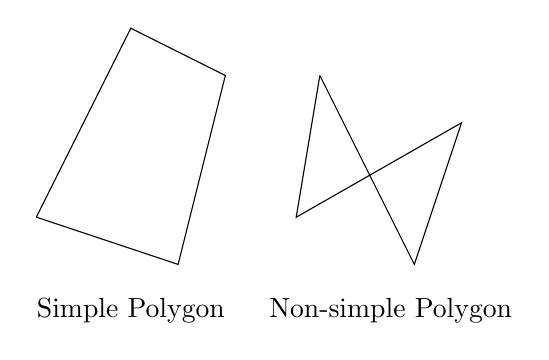
\begin{tikzpicture}[scale=0.6]
					\draw (0, 0) -- (3, -1) -- (4, 3) -- (2, 4) -- (0, 0);
					\draw (6, 3) -- (8, -1) -- (9, 2) -- (5.5, 0) -- (6, 3);
					\node at (2, -1.5) [below] {Simple Polygon};
					\node at (7.5, -1.5) [below] {Non-simple Polygon};
				\end{tikzpicture}
			\end{figure}\\
			Polygons are basic building blocks in most geometric applications. It can model arbitrarily complex shapes, and apply simple algorithms and algebraic representation/manipulation.
			
		\section{Triangulation}
			\framebox{\textbf{Def:}} \textbf{Triangulation} is to partition polygon $P$ into non-overlapping triangles using diagonals only. It reduces complex shapes to collection of simpler shapes. Every simple $n$-gon admits a triangulation which has $n-2$ triangles.\\
			\begin{figure}[h!]
				\centering
				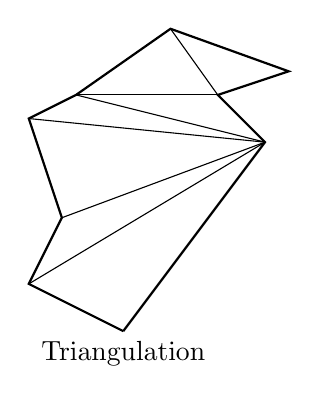
\begin{tikzpicture}[scale=0.6]
					\draw [thick] (0, 0) -- (3, 4) -- (2, 5) -- (3.5, 5.5) -- (1, 6.4) -- (-1, 5) -- (-2, 4.5) -- (-1.3, 2.4) -- (-2, 1) -- (0, 0);
					\draw (-2, 1) -- (3, 4);
					\draw (-1.3, 2.4) -- (3, 4);
					\draw (-2, 4.5) -- (3, 4);
					\draw (-1, 5) -- (3, 4);
					\draw (-1, 5) -- (2, 5);
					\draw (2, 5) -- (1, 6.4);
					\node at (0, 0) [below] {Triangulation};
				\end{tikzpicture}
			\end{figure}\\
			\framebox{\textbf{Theorem:}} Every polygon has a triangulation\\  
			\framebox{\textbf{Lemma:}} Every polygon with more than three vertices has a diagonal.\\
			\framebox{\textbf{Proof:}}(by Meisters, 1975) Let $P$ be a polygon with more than three vertices. Every vertex of a $P$ is either \textit{convex} or \textit{concave}. W.L.O.G.(any polygon must has convex corner) Assume $p$ is a convex vertex. Denote the neighbors of $p$ as $q$ and $r$. If $\bar{qr}$ is a diagonal, done, and we call $\triangle{pqr}$ is an \textit{ear}. If $\triangle{pqr}$ is not an ear, it means at least one vertex is inside $\triangle{pqr}$, assume among those vertexes inside $\triangle{pqr}$, $s$ is a vertex closest to $p$, then $\bar{ps}$ is a diagonal. 
			
		\section{Art Gallery Theorem}
			\framebox{\textbf{Problem:}} The floor plan of an art gallery modeled as a simple polygon with $n$ vertices, there are guards which is stationed at fixed positions with 360 degree vision but cannot see through the walls. How many guards does the art gallery need for the security? (Fun fact: This problem was posted to Vasek Chvatal by Victor Klee in 1973)\\
			\framebox{\textbf{Theorem:}} Every $n$-gon can be guarded with $\lfloor \frac{n}{3} \rfloor$ vertex guards\\
			\framebox{\textbf{Lemma:}} Triangulation graph can be 3-colored.\\
			\framebox{\textbf{Proof:}} \\
			- $P$ plus triangulation is a planar graph\\
			- 3-coloring means there exist a 3-partition for vertices that no edge or diagonal has both endpoints within the same set of vertices.\\
			- Proof by Induction:\\
			\indent - Remove an ear (there will always exist ear) \\
			\indent - Inductively 3-color the rest\\
			\indent - Put ear back, coloring new vertex with the label not used by the boundary diagonal.

		\section{Triangulation Algorithms}

		\section{Shortest Path}


